\chapter{Introduction}

\section{Course Structure \& Logistics}
\subsection{Structure}
\twosplit{
    \begin{center}
        \begin{tikzpicture}
        \clip (0,0)  circle (2cm) ;
        \node[anchor=center] at (0,-0.5) {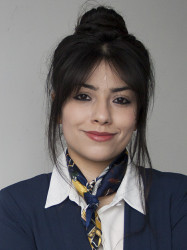
\includegraphics[width=4.5cm]{introduction/images/azalea_raad.jpg}}; 
        \end{tikzpicture}
        \centerline{\textbf{Dr Azalea Raad}}
    \end{center}
    \textbf{Theory} For weeks 2 $\to$ 5:
    \begin{itemize}
        \item Intro to synchronisation paradigms (mutual exclusion, readers-writers, producer-consumer)
        \item Low-level concurrent semantics (sequential consistency, Intel-x86)
        \item High-level concurrent semantics (concurrent objects, linearisability)
        \item Transactional memory (serialisability)
    \end{itemize}
}{
    \begin{center}
        \begin{tikzpicture}
        \clip (0,0)  circle (2cm) ;
        \node[anchor=center] at (-.1,0.0) {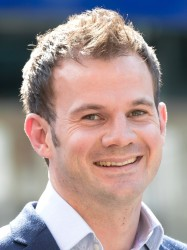
\includegraphics[width=4.5cm]{introduction/images/alastair_donaldson.jpg}}; 
        \end{tikzpicture}
        \centerline{\textbf{Prof Alastair Donaldson}}
    \end{center}
    \textbf{Practical} For weeks 5 $\to$ 8:
    \begin{itemize}
        \item Threads and locks in C++
        \item Implementing locks
        \item Concurrency in Haskell
        \item Race-free concurrency in Rust
        \item Dynamic data-race detection
    \end{itemize}
}

\subsection{Extra Materials}
\begin{center}
    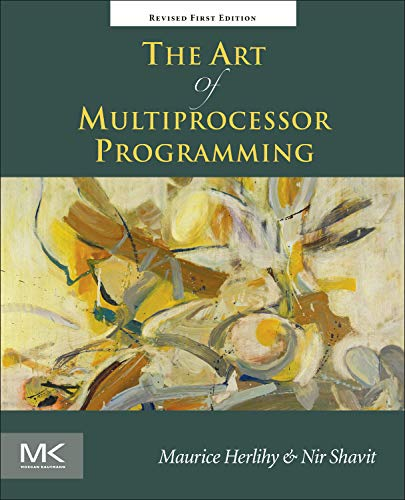
\includegraphics[height=6cm]{introduction/images/the_art_of_multicore_programming.jpg}
    \\ \href{https://cs.ipm.ac.ir/asoc2016/Resources/Theartofmulticore.pdf}{\textbf{The Art of Multiprocessor Programming}}
    \\ About $65\%$ of the theory course.
\end{center}


\section{Preface for Concurrency}
\subsection{Moore's Law}
\begin{definitionbox}{Moore's Law}
    An empirical (supported by observation) law that states the density of transistors in an integrated circuit
    will double approximately every two years.
    \begin{itemize}
        \item The observation is named after Gordon Moore (co-founder and later CEO of Intel).
        \item This law no longer holds, and sequential performance improvements have declined.
    \end{itemize}
\end{definitionbox}

\begin{definitionbox}{Dennard/MOSFET Scaling}
    \[\text{Power} \propto \text{Transistor Size}\]
    A scaling law stating that as transistor density increases, the power requirements stay constant. 
    \begin{itemize}
        \setlength\itemsep{0em}
        \item Increasing transistor density results in power staying constant (less power per transistor) and lower circuit delay. 
        \item This allows for higher switching frequency $\Rightarrow$ higher clocks frequencies $\Rightarrow$ better sequential performance).
    \end{itemize}
\end{definitionbox}

\begin{center}
    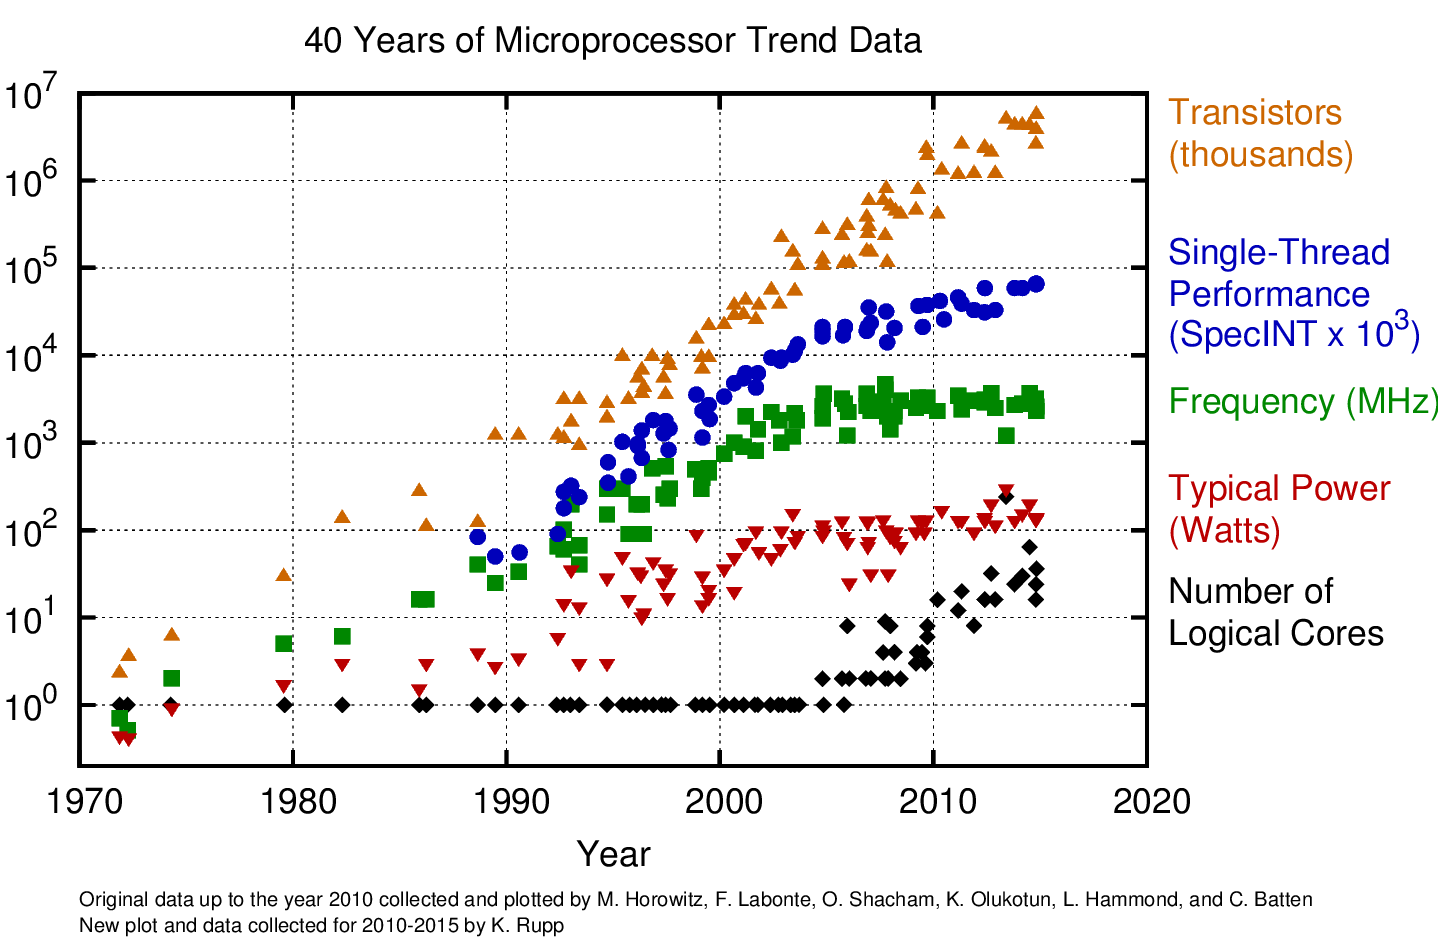
\includegraphics[width=.9\textwidth]{introduction/images/moores_law_graph.png}
\end{center}
The performance improvements typically expected yearly (moore's law and Dennard scaling) no longer apply.
\begin{itemize}
    \item Sequential (Single-Thread) performance improvements have declined.
    \item Parallelism is being exploited to improve performance (uniprocessors are virtually extinct).
    \item Shared-memory multiprocessor systems have lost out to multicore processors.
\end{itemize} 

\begin{definitionbox}{Amdahl's Law}
    \[S_{\text{latency}}(s) = \cfrac{1}{(1-p)+ \cfrac{p}{s}} \text{ where } p = \text{parallel portion} \text{ and } s = \text{threads}\]
    Amdahl's law describes the speedup of a program, associated with the number of threads.
    \begin{itemize}
        \item Can be applied to other resources.
        \item Versions of the equation exist for different proportions using different numbers of threads.
        \item As the number of threads increases the sequential part of the program becomes a bottleneck. 
    \end{itemize}
\end{definitionbox}

\subsection{Concurrency Difficulties}
Writing correct, concurrent code is difficult.
\begin{definitionbox}{race Condition}
    A potential for a situation where the result of a program depends on the non-deterministic timing or interleaving of threads.
    \begin{itemize}
        \item Where multiple threads access data (non-atomically) and at least one writes.
        \item Where a lack of enforced ordering on some events causes differing results (e.g output to user)
    \end{itemize}
    Race conditions can be intentional, where the result of the program is intended to be based off some non-deterministic input.
    \begin{itemize}
        \item Which thread gets to write first?
        \item Which process is allowed to write to a file?
    \end{itemize}
\end{definitionbox}
\begin{itemize}
    \item A process can have multiple threads executing in parallel.
    \item Cannot determine at compile time the relative speed of execution of threads (many delays are unpredictable; cache misses, page faults, interrupts).
    \item Cannot predict how long threads will be blocked (e.g I/O) or when threads will be scheduled (or use up their time quantum).
\end{itemize}
Hence we must use synchronisation mechanisms to regulate accesses to shared data that can result in a race condition.

\subsection{OS Concepts}
\begin{minipage}{.3\textwidth}
    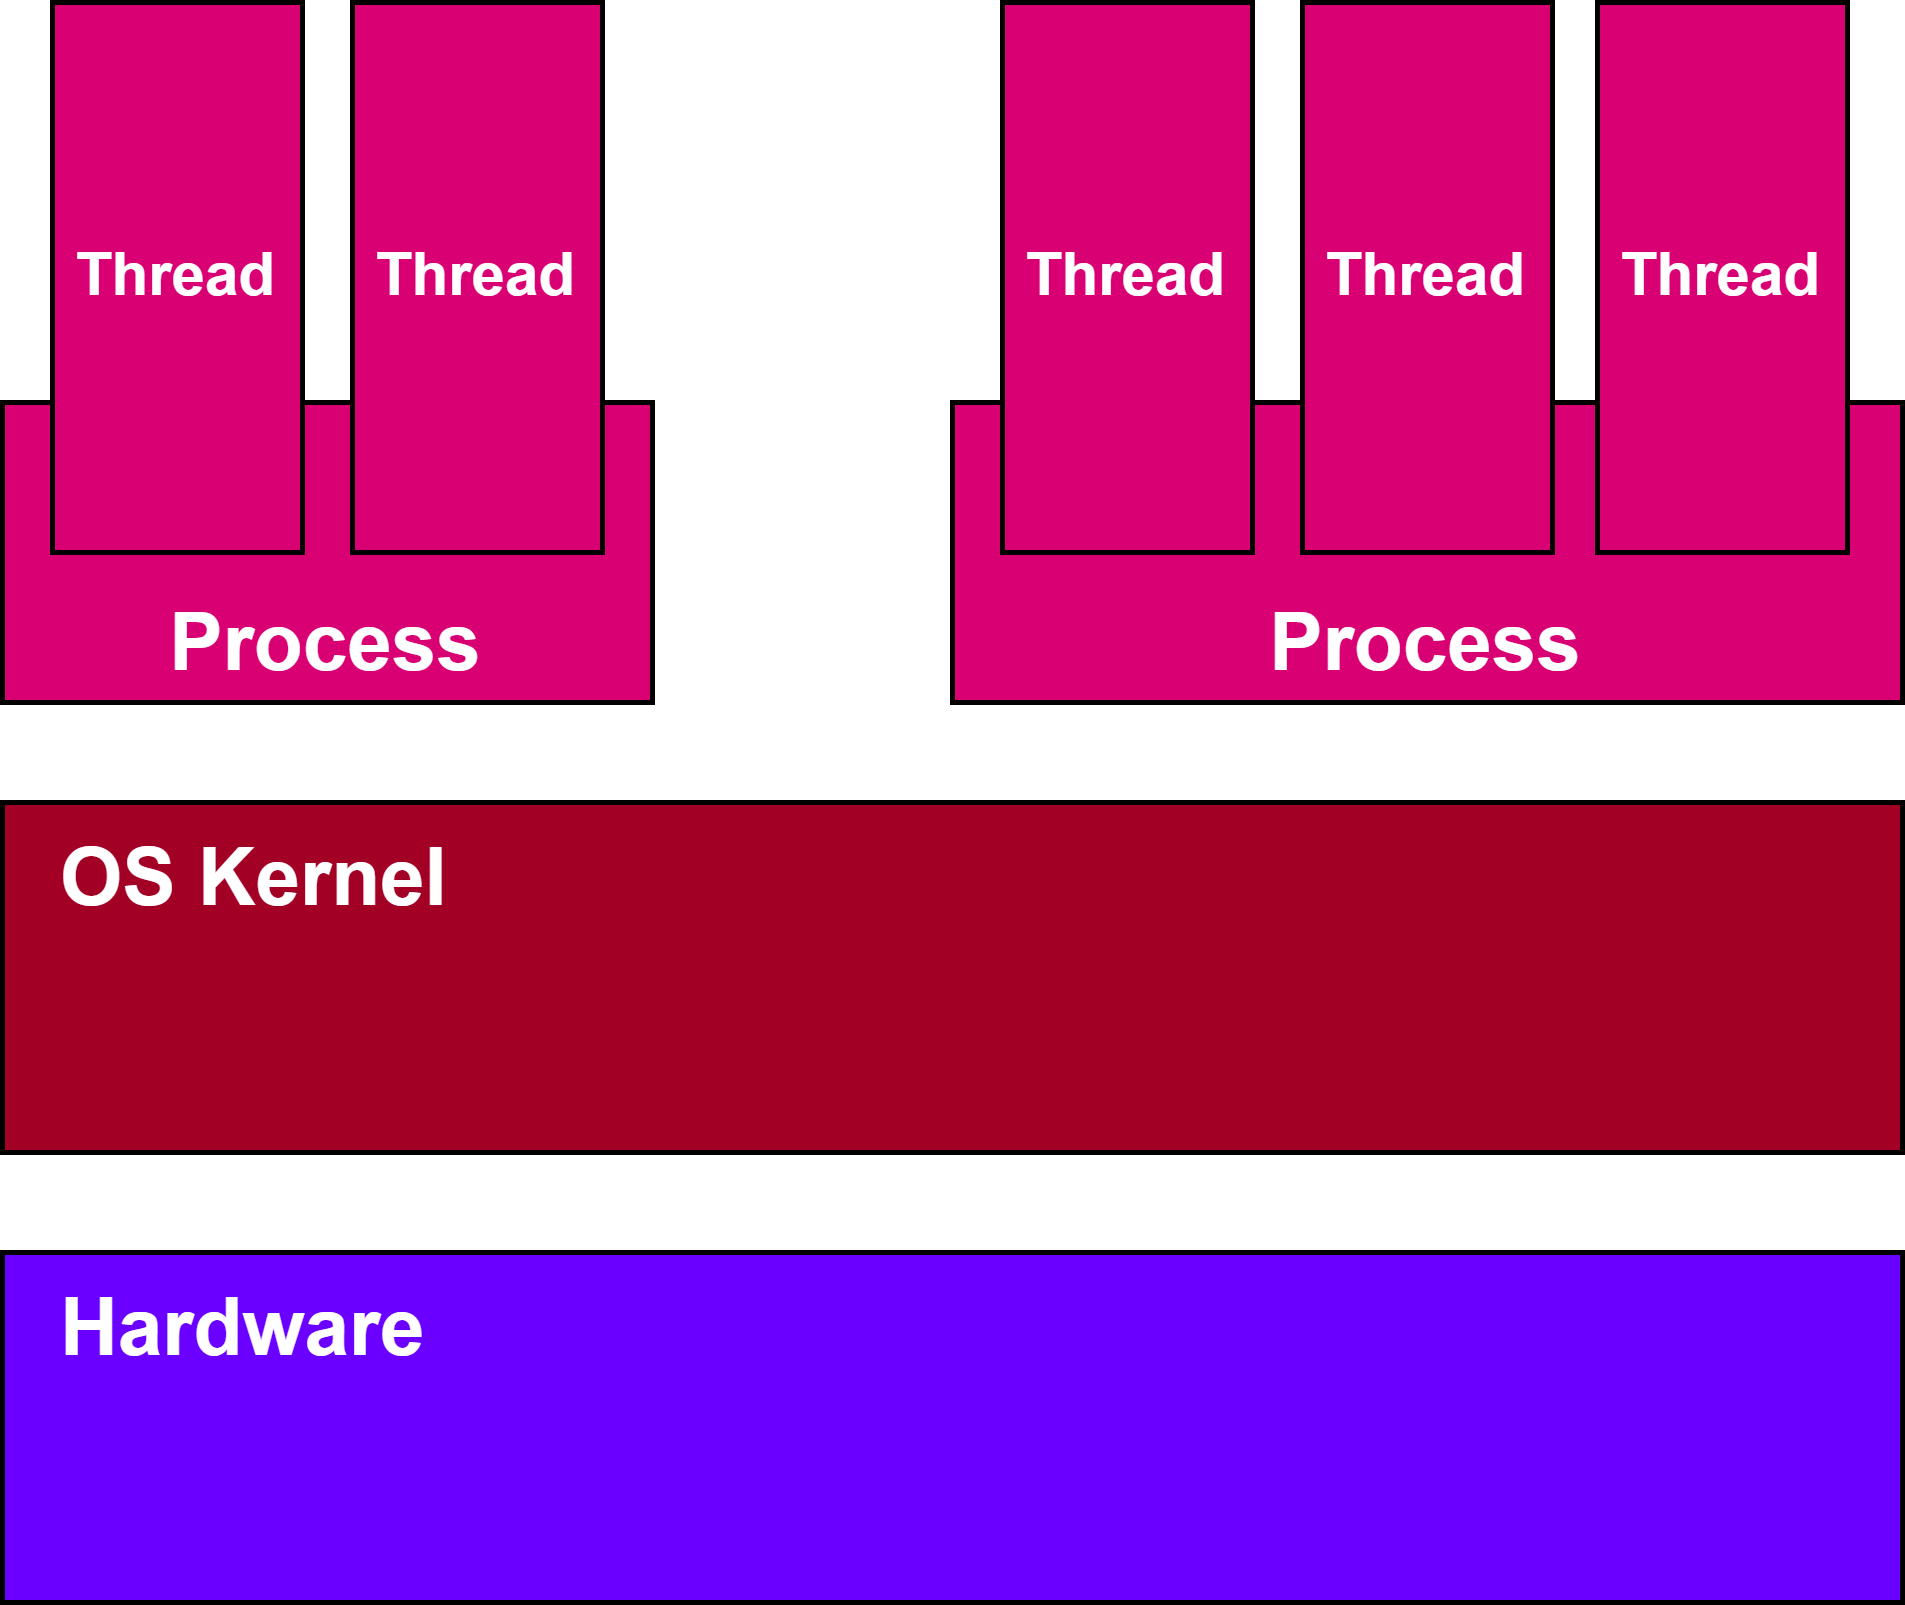
\includegraphics[width=\textwidth]{introduction/images/os_stack.drawio.png}    
\end{minipage}
\hfill
\begin{minipage}{.68\textwidth}
    \begin{itemize}
        \item Operating system provides process and thread abstractions.
        \item A process contains one or more threads (streams of instructions being executed).
        \item A process has its own address space, all threads in the process share this address space.
        \item The OS kernel contains a scheduler which schedules processes \& their threads.
    \end{itemize}
\end{minipage}

